\documentclass[14pt]{beamer}
\usepackage{fontspec}
\usepackage{color}
\usepackage{minted}

%% These fonts are non-free.
%% Comment out the lines if you don't have them.
\setmainfont{Equity Text A}
\setsansfont{Concourse T3}
\setmonofont{Triplicate T4}

\definecolor{bgcolor}{RGB}{20,25,28}
\setbeamercolor{background canvas}{bg=bgcolor}
\setbeamercolor{normal text}{fg=white}
\setbeamercolor{itemize item}{fg=white}
\setbeamertemplate{itemize items}[circle]
\usemintedstyle{monokai}

\renewcommand{\theFancyVerbLine}{\color{darkgray}\large \oldstylenums{\arabic{FancyVerbLine}}}
\newcommand{\toptitle}[1]{
  {\huge #1} \\
  \vspace{0.2cm}
}
\renewcommand{\subtitle}[1]{
  {\large #1} \\
  \vspace{0.2cm}
}

\begin{document}
\begin{frame}
  \begin{center}
    
\includegraphics[height=4cm]{avatar.png}\\
    \vspace{0.2cm}
    {\Large Nicolas Hafner} \\
    \vspace{0.2cm}
    {\Huge @Shinmera} \\
    \vspace{0.2cm}
    \url{https://everything.shinmera.com}
  \end{center}
\end{frame}

\begin{frame}
  \toptitle{GUIs in Lisp}
  Common Lisp Native GUI Toolkits
  \begin{itemize}
  \item McCLIM
    \pause
  \item ... that's about it.
  \end{itemize}
  \vspace{0.5cm}

  \pause
  Other languages offer alternatives
  \begin{itemize}
  \item Qt
  \item Gtk
  \item Ltk
  \item Swing
  \item etc.
  \end{itemize}
\end{frame}

\begin{frame}
  \toptitle{Qt}
  \begin{itemize}
  \item Gigantic
  \item Well-documented
  \item Cross-platform
    \pause
  \item Written in C++
  \end{itemize}
  \vspace{0.5cm}

  \pause
  \subtitle{Smoke}
  \begin{itemize}
  \item Generates C wrappers for C++
  \item Can also handle Qt
  \end{itemize}
\end{frame}

\begin{frame}
  \toptitle{CommonQt}
  \begin{itemize}
  \item Runs with CCL, SBCL on Windows, Mac, Linux
  \item Actively supported
  \item It Just Works\texttrademark
    \pause
  \item Awkward to use
  \end{itemize}
\end{frame}

\begin{frame}
  \toptitle{An Example}
  \begin{center}
    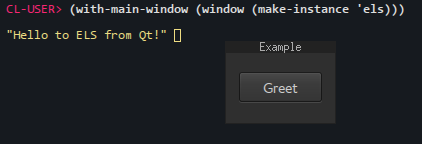
\includegraphics[height=3cm]{example.png}
  \end{center}
\end{frame}

\begin{frame}[fragile]
  \fontsize{9pt}{9pt}
\begin{minted}{common-lisp}
(defclass els () 
  ((button))
  (:metaclass qt-class)
  (:qt-superclass "QWidget")
  (:slots ("buttonPressed()" button-pressed)))

(defmethod initialize-instance :after ((els els) &key)
  (new els)
  (#_setWindowTitle els "Example")
  (let ((button (#_new QPushButton "Greet" els))
        (layout (#_new QHBoxLayout els)))
    (setf (slot-value els 'button) button)
    (connect button "released()" 
                els "buttonPressed()")
    (#_addWidget layout button)))

(defmethod button-pressed ((els els))
  (print "Hello to ELS from Qt!"))
\end{minted}
\end{frame}

\begin{frame}[fragile]
  \fontsize{9pt}{9pt}
\begin{minted}{common-lisp}
(define-widget els (QWidget)
  ())

(define-subwidget (els button) (q+:make-qpushbutton "Greet"))

(define-subwidget (els layout) (q+:make-qhboxlayout els)
  (q+:add-widget layout button))

(define-slot (els button-pressed) ()
  (declare (connected button (released)))
  (print "Hello to ELS from Qt!"))
\end{minted}
\end{frame}

\begin{frame}
  \toptitle{Qtools}
  \begin{itemize}
  \item Started out as collection of utilities
  \item Grew into a full convenience layer
  \item Now makes writing GUIs look normal
  \item Tries to take care of C++ garbage
  \item And all sorts of other things
  \end{itemize}
\end{frame}

\begin{frame}
  \begin{center}
    \hskip1.2cm
\includegraphics[height=3cm]{qtools-logo.png} \\
    {\bfseries \url{https://shinmera.github.io/qtools}} \\
    \vspace{0.3cm}
    {\Large Available on Quicklisp}
  \end{center}
\end{frame}
\end{document}

%%% Local Variables:
%%% mode: latex
%%% TeX-command-extra-options: "-shell-escape"
%%% TeX-master: t
%%% TeX-engine: luatex
%%% End:
